\chapter{Použitý model}

\begin{figure}
	\caption{Části adresy URL}\label{url_parts}
	\centering
	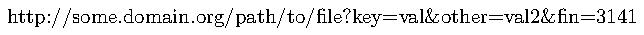
\includegraphics{images/url/url.pdf}
\end{figure}

\begin{figure}
	\caption{Model adresy URL}\label{url_model}
	\centering
	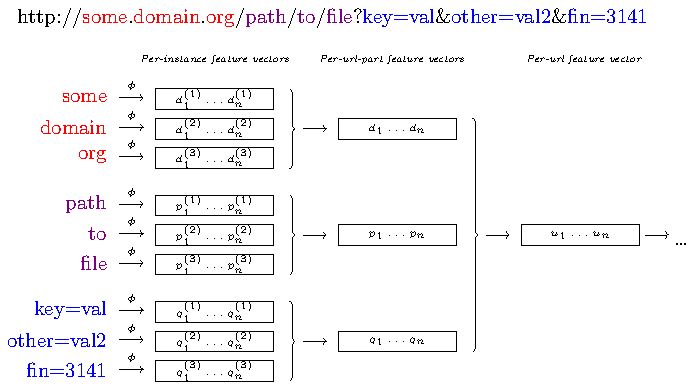
\includegraphics{images/model/model.pdf}
\end{figure}

\section{Řešená úloha}
Řešíme úlohu vyhovující formalismu, popsaném v \ref{used_formalism}, ke klasifikaci síťových spojení. Cílem je navrhnout klasifikační funkci, která pro danou vstupní URL adresu (\textit{\textenglish{uniform resource locator}}, srov. \cite{berners-lee_uniform_1994}) rozhodne, zda spojení mířící na takovouto adresu pochází z běžné aktivity uživatele-klienta, či zda se jedná o spojení, které vytvořil nějaký nežádoucí software. Pro tento účel nejprve rozložíme URL na tři části, a to sice doménu, (\textit{\textenglish{domain}}), cestu (\textit{\textenglish{path}}) a dotaz (\textit{\textenglish{query}}). Na obrázku \ref{url_parts} vidíme toto rozložení na příkladu, červeně je vyznačená doména, fialově cesta a modře dotaz. Dále pak každou část adresy rozdělíme na několik podčástí. Doménu dělíme podle znaku \enquote{.} (tečka), tedy podle jednotlivých úrovní domén. Cestu dělíme podle znaku \enquote{/} (lomítko), tedy na jednotlivé adresáře a soubory. Dotaz dělíme podle znaku \enquote{\&} (ampersand), tedy na páry klíč-hodnota. Na všechny takto vytvořené aplikujeme nějakou funkci \( \psi : U^* \to \mathbb R^n \), kde \( U \) je abeceda všech znaků unicode. Tím získáme prostor vstupních objektů jako
\begin{equation}
	\BPspace X = \psi \left( U^* \right) \subset \mathbb R^n
\end{equation}
V prostoru \( X \) jsou tedy vektory příznaků všech částí adresy. Zkonstruujeme prostor \( \BPspace B_1 \) tak, že každá taška v \( \BPspace B_1 \) odpovídá příznakům jedné části (domény, cesty nebo dotazu) jedné adresy. Potom podle formalismu nastíněného v \ref{used_formalism} můžemee najít vkládající funkci \( \phi_1 : \BPspace B_1 \to \BPspace X \). Dále pak konstruujeme prostor \( \BPspace B_2 \) tak, že každá taška v \( \BPspace B_2 \) odpovídá příznakům jedné adresy, tedy platí
\begin{equation}
	\left( \forall b \in \BPspace B_2 \right) \left( \left| b \right| \leq 3 \right)
\end{equation}

Znovupoužitím formalismu z \ref{used_formalism} můžeme definovat vkládající funkci \( \phi_2 : \BPspace B_2 \to \BPspace X \).

\section{Model}

\section{Trénovací a testovací data}

